\chapter{Mécanique ondulatoire} % (fold)
\label{chap:Mécanique ondulatoire}

\begin{tcolorbox}
Équation de Schrödinger

\begin{itemize}

    \item Équation de Schrödinger dépendante du temps : en 3D et 1D
    \item Conservation de la norme
    \item Équation de Schrödinger indépendante du temps : condition et forme — État stationnaire
    \item Courant de probabilité et équation de continuité
    \item Exemple : particule libre (V = 0)

\end{itemize}
\end{tcolorbox}

\newpage
\section{Équation de Schrödinger} % (fold)

\begin{tcolorbox}
Équation de Schrödinger
\begin{itemize}

    \item Équation de Schrödinger dépendante du temps : en 3D et 1D 
    \item Conservation de la norme 
    \item Équation de Schrödinger indépendante du temps : condition et forme — État stationnaire 
    \item Courant de probabilité et équation de continuité

\end{itemize}
\end{tcolorbox}

\begin{note}{}{}
L'expérience du \textbf{Principe fondamentale dynamique} démontre que 
\begin{itemize}

    \item Pour un système de $N$ particule : 
      \begin{equation}
        \overrightarrow{F_i} = \overrightarrow{\nabla} V_i = m_i \frac{\mathrm{d} ^{2} \overrightarrow{r_i}}{\mathrm{d} t ^{2}} 
      \end{equation}

    \item Équation d'évolution est une équation différentielle de l'ordre 2. Si on connaît les \underline{positions initiales} et les \underline{vitesses initiales}, on connâit l'évolution temporelle du système.

\end{itemize}

Le système quantique est décrit par la fonction d'onde, et l'équation d'évolution est équation différentielle d'ordre 1.
\end{note}

\subsection{Forme générale} % (fold)

\subsubsection{Équation de Schrödinger 3D et 1D} % (fold)

\begin{Theorem}{Équation de Schrödinger}{}
On pose $V(M,t)$ (réelle) la \underline{énergie potentielle} dépendant éventuellement du temps.
Le postulat fondamental : la fonction d'onde vérfie
\begin{equation}
  - \frac{\hbar ^{2}}{2m}  \Delta \psi(M,t) + V(M,t) \psi(M,t) = i \hbar \frac{\partial \psi}{\partial t} (M,t)
\end{equation}

Dans le cas 1D : 
\begin{equation}
  - \frac{\hbar ^{2}}{2m}  \frac{\partial  ^{2} \psi(x,t)}{\partial x ^{2}}  + V(x,t) \psi(x,t) = i \hbar \frac{\partial \psi}{\partial t} (x,t)
\end{equation}
\end{Theorem}

Rappel : Dans la partie \ref{sub: Application en mécanique}, on a déjà vu que : 
\begin{equation}
  E_m = \frac{ \| \overrightarrow{p} \| ^{2}}{2m} + V(x,t)\to \hat{H} = - \frac{\hbar ^{2}}{2m} \Delta + \hat{V}(M,t)
\end{equation}

\begin{Theorem}{}{}
Avec l'\textbf{opérateur hamiltonien} 
\begin{equation}
  \hat{H} = - \frac{\hbar ^{2}}{2m}  \frac{\partial ^{2}}{\partial x ^{2}}  + V(x,t)
\end{equation}

On obtient 
\begin{equation}
  \color{red}\boxed{\hat{H} \psi = i \hbar \frac{\partial \psi}{\partial t} }
\end{equation}
\end{Theorem}


\subsection{Propriétés} % (fold)

% section Propriété (end)


\subsubsection{Linéarité} % (fold)
\label{sub:Linéarité}

Elle est compatible avec le \textbf{principe de superpostion} : Si $\psi_1$ et $\psi_2$ sont des solutions, alors toute combinaison linéaire est également solution.
% subsection Linéarité (end)

\subsubsection{Conservation de la norme} % (fold)
\label{sub:Conservation de la norme}

\begin{Theorem}{}{}
Une fonction $\psi(M,t)$ vérifiant l'équation de Schrödinger garde une norme constante.
\end{Theorem}

\begin{myproof}{}{}
  Posons 
  \begin{equation}
    N(t) = \int_{- \infty}^{+ \infty} | \psi(x,t) | ^{2} \mathrm{d} x = \int_{- \infty}^{ + \infty} \psi ^{*}(x,t) \psi(x,t)\mathrm{d}x
  \end{equation}

  Donc, 
  \begin{align}
    \frac{\mathrm{d}N}{\mathrm{d}t} &= \int_{- \infty}^{+ \infty} \frac{\partial \psi ^{*}}{\partial t} \psi \mathrm{d} x + \int_{- \infty}^{+ \infty} \psi ^{*} \frac{\partial \psi}{\partial t} \mathrm{d}x \\ 
                                    &= 2 \mathrm{Re}\left( \int_{- \infty}^{+ \infty} \frac{\partial  \psi ^{*}}{\partial t} \psi \mathrm{d}x \right) \quad (1 ^{*} = 2,\; \text{utiliser 2D coor.})
                                \\ &= 2 \mathrm{Re} \left( \int_{- \infty}^{+ \infty} \frac{
                                        i
                                    }{\hbar} \left( - \frac{\hbar ^{2}}{2m} \frac{\partial ^{2} \psi ^{*}}{\partial x ^{2}} + V(x,t) \psi ^{*} \right) \psi \mathrm{d}x \right) \\ 
                                    &= - \frac{\hbar}{m} \mathrm{Re} \left( i \int_{- \infty}^{+ \infty} \left( \frac{\partial ^{2}\psi ^{*}}{\partial x ^{2}}  \right) \psi \mathrm{d}x \right)\; (V(x,t) \text{ disparaît car la partie imag. pur}) \\ 
                                    &=  - \frac{\hbar}{m} \mathrm{Re} \left( i \times \left[ \psi \frac{\partial \psi ^{*}}{\partial x}  \right]_{- \infty} ^{+ \infty} - i \times \int_{- \infty}^{+ \infty} | \frac{\partial \psi}{\partial x} | ^{2}\mathrm{d}x \right) \;(\text{IPP})
  \end{align}

  La première terme est nulle car la fonction d'onde et ses dérivées sont dominées par des fonctions intégrables, donc nécessairement tendent vers 0 à l'infini.

  La deuxième terme est nulle car c'est la partie imaginaire. 

  Enfin, 
  \begin{equation}
    \frac{\mathrm{d}N}{\mathrm{d}t}  = 0
  \end{equation}
\end{myproof}


\subsubsection{Justification d'une onde de de Broglie} % (fold)
\label{sub:Justification d'une onde de de Broglie}
Pour une \underline{particule libre} ($V=0$) décrite par une onde de Broglie unidimensionnelle : 
\begin{equation}
  \psi = A \exp \frac{i}{\hbar}  (p x -Et)
\end{equation}

Nous avons 
\begin{equation}
  i \hbar \frac{\partial \psi}{\partial t} =  E \psi, \; - \frac{\hbar ^{2}}{2m} \frac{\partial ^{2}\psi}{\partial x ^{2}}  = \frac{p ^{2}}{2m}  \psi
\end{equation}

Les ondes de de Broglie vérifient dans le mesure où l'énergie de la particule est donné par
\begin{equation}
  E = \frac{p ^{2}}{2m} 
\end{equation}
% subsection Justification d'une onde de de Broglie (end)



% subsection Conservation de la norme (end)
% section Forme générale (end)

\subsection{Équation de Schrödinger indépendante du temps} % (fold)
\label{sec:Équation de Schrödinger indépendante du temps}

% section Équation de Schrödinger indépendante du temps (end)

\subsubsection{Forme générale} % (fold)
\label{sub:Forme générale}

Nous considérons des situations où l'\underline{énergie potentielle est indépendant du temps}, pour que $\hat{H}$ indépendant du temps : 
\begin{equation}
  - \frac{\hbar ^{2}}{2m}  \Delta \psi(M,t) + V(M) \psi(M,t) = i\hbar \frac{\partial \psi}{\partial t} (M,t)
\end{equation}
% subsection Forme générale (end)

On obtient une expression \underline{séparant des variables} : 
\begin{equation}
  \psi(M,t) = \widetilde{\psi}(M) \exp \left( - \frac{iEt}{\hbar}  \right)
\end{equation}

avec
\begin{itemize}

    \item $E$ l'énergie du système 
    \item $\widetilde{\psi}(M)$ l'\textbf{état stationnaire} qui sont les \textbf{états propres} de $\hat{H}$, les énergies associées sont des \textbf{valeurs propres de l'hamiltonien}.

\end{itemize}

Les deux satisfait : 

\begin{Theorem}{Équation de Schrödinger indépendante du temps (ou stationnaire)}{}
\begin{equation}
  - \frac{\hbar ^{2}}{2m} \Delta \widetilde{\psi}(M) + V(M) \widetilde{\psi}(M) = E  \widetilde{\psi}(M) \quad\text{ ou } \quad \color{red} \boxed{\hat{H} \widetilde{\psi} = E \widetilde{\psi}}
\end{equation}
\end{Theorem}


\subsubsection{État stationnaire} % (fold)
\label{sub:État stationnaire}

\begin{itemize}

    \item Densité de probabilité indépendante du temps 
      \begin{equation}
        | \psi(M,t) | ^{2} = | \widetilde \psi(M) | ^{2}
      \end{equation}

    \item La valeur moyenne de $A$ pour un système dans l'état stationnaire est indépendant du temps 
      \begin{equation}
        \langle A \rangle =  \langle \psi | \hat{A} | \psi  \rangle = \int_{}^{} \psi ^{*}(M,t) \hat{A} \psi ^{*}(M,t) \mathrm{d}V = \int_{}^{} \widetilde{\psi} ^{*}(M) \hat{A} \widetilde{\psi}(M) \mathrm{d}V
      \end{equation}

\end{itemize}
% subsection État stationnaire (end)

% section  (end)

\subsection{Résoudre une équation de Schrödinger} % (fold)
\label{sub:Résoudre une équation de Schrödinger}

La solution générale de $\hat{H} \psi = i \hbar \frac{\partial  \psi}{\partial t}$ est la combinaison linéarie des solutions de l'équation de Schrödinger indépendante du temps $\hat{H} \widetilde \psi = E \widetilde \psi$, avec chaque état stationnaire correspond à un niveau d'énergie.
\begin{equation}
  \boxed{\psi(M,t) = \sum_{n}^{}C_n \widetilde{\psi}_n(M) \exp \left( - \frac{iE_nt}{\hbar}  \right)}
\end{equation}

Avec les coefficients : 
\begin{equation}
  C_n = c_n(t = 0) = \int_{0}^{a} \widetilde \psi _n ^{*}(x) \times \widetilde \psi(x, t = 0) \mathrm{d}x = \langle \widetilde \psi _n | \widetilde \psi (x, t = 0)\rangle 
\end{equation}

Exemple : à voir.
% subsection Résoudre une équation de Schrödinger (end)

\subsection{Courant de probabilité} % (fold)
\label{sec:Courant de probabilité}

\begin{itemize}
    \item Rappel en électromagnétisme et en mécanique de fluide, la densité de courant a une expression : $\overrightarrow{j} = \rho \overrightarrow{v}$

    \item La vitesse de la particule associée à l'opérateur et son moyenne : 
      \begin{equation}
        \hat{\overrightarrow{v}} = \frac{\hat{\overrightarrow{p}}}{m}  \implies \langle \overrightarrow{v} \rangle = \iiint \psi ^{*} \frac{\hat{\overrightarrow{p}}}{m} \psi \mathrm{d} V_M
      \end{equation}

    \item Donc de même, définissions la quantité 
      \begin{equation}
        \boxed{        \overrightarrow{J} = \mathrm{Re} \left( \frac{1}{m} \psi ^{*} \hat{\overrightarrow{p}} \psi \right)} = \frac{\hbar}{2im} \left( \psi ^{*} \overrightarrow{\mathrm{grad}} \psi - \psi \overrightarrow{\mathrm{grad}} \psi ^{*}\right)
      \end{equation}

      \begin{myproof}{En sachant que $\mathrm{Re}(a) = \frac{a+ a ^{*}}{2} $}{}
      \begin{equation}
        \overrightarrow{J} = \frac{- \hbar}{m} \mathrm{Re}(i \psi ^{*} \overrightarrow{\mathrm{grad}} \psi) = \frac{- \hbar}{2m}  (i \psi ^{*} \overrightarrow{\mathrm{grad}} \psi - i \psi \overrightarrow{\mathrm{grad}} \psi ^{*})
      \end{equation}
      \end{myproof}

    \item Si la fonction d'onde est réelle, le courant de probabilité est nul.  
      \begin{myproof}{}{}
      Seulement $\hat{\overrightarrow{p}}$ contenant $i$, et les autres quantités sont réelles.
      \end{myproof}

      
    \item Exemple d'onde de de Broglie : 
\begin{equation}
  \psi(M,t) = C \exp \left( \frac{i}{\hbar} ( \overrightarrow{p}. \overrightarrow{OM}- Et) \right) \implies \overrightarrow{j} = \frac{|\psi| ^{2}}{m}  \overrightarrow{p} = \rho(M,t) \overrightarrow{v}
\end{equation}

\begin{myproof}{}{}
\begin{align}
  \overrightarrow{j} &= \mathrm{Re} \left( \frac{1}{m}  \psi ^{*} \hat{ \overrightarrow{p}} \psi \right) \\
                     &= \mathrm{Re} \left( \frac{1}{m} \psi _{\overrightarrow{p_0}} ^{*} \times (-i \hbar \overrightarrow{\mathrm{grad}} \psi _{\overrightarrow{p_0}}) \right) \\
                     &= \mathrm{Re} \left( \frac{1}{m} \psi _{\overrightarrow{p_0}} ^{*} \times \left(-i \hbar \frac{i}{\hbar} \overrightarrow{p_0} . \psi _{\overrightarrow{p_0}}\right) \right) \\
                     &= |A| ^{2} \times \frac{\overrightarrow{p_0}}{m} 
\end{align}
\end{myproof}




    \item Conservation de conservation de la densité de probabilité, analogue aux équations de conservation de charge et de masse : 
      \begin{equation}
        \boxed{\frac{\partial \rho}{\partial t} + \mathrm{div} \overrightarrow{J} = 0}
      \end{equation}

    \begin{myproof}{}{}
     On le divise dans deux parties : 
     \begin{itemize}

         \item Permier terme 

           D'après l'équation de Schrödinger, 
           \begin{gather}
             \frac{\partial }{\partial t} \psi = \frac{1}{i \hbar}  \left( - \frac{\hbar ^{2}}{2m}  \Delta \psi + V \psi \right) \\
             \frac{\partial }{\partial t} \psi ^{*} = \frac{-1}{i \hbar}  \left( - \frac{\hbar ^{2}}{2m}  \Delta \psi ^{*} + V \psi  ^{*}\right)
           \end{gather}

           Donc
           
           \begin{align}
             \frac{\partial \rho}{\partial t} &= \frac{\partial }{\partial t}  ( \psi ^{*} \psi) = \psi ^{*} \frac{\partial \psi}{\partial t} + \psi \frac{\partial \psi ^{*}}{\partial t}  \\
                                              &= \frac{1}{i \hbar}  \times \left[ - \frac{\hbar ^{2}}{2m} (\psi ^{
                 *
             } \Delta \psi - \psi \Delta \psi ^{*}) \right] \\ 
             &= - \frac{\hbar}{2im} (\psi ^{*} \Delta \psi - \psi \Delta \psi ^{*})
           \end{align}

          \item Deuxième terme (Rappel : $\overrightarrow{\nabla} ^{2} = \Delta$)

            \begin{align}
              \overrightarrow{\nabla}. \overrightarrow{j} &= \frac{\hbar}{2im} \overrightarrow{\nabla}.( \psi ^{*} \overrightarrow{\nabla} \psi - \psi \overrightarrow{\nabla} \psi ^{*}) \\
                                                          &= \frac{\hbar}{2im}  ( \overrightarrow{\nabla}\psi ^{*}. \overrightarrow{\nabla} \psi + \psi ^{*} \overrightarrow{\nabla} ^{2} \psi - \overrightarrow{\nabla} \psi. \overrightarrow{\nabla} \psi ^{*} - \psi \overrightarrow{\nabla} ^{2} \psi ^{*})
            \end{align}

     \end{itemize}
    \end{myproof}

    

      

\end{itemize}
% section Courant de probabilité (end)
% chapter Équation de Schrödinger (end)

\newpage
\section{Particule libre} % (fold)
\label{sec:Particule libre}

\subsection{Parquet d'ondes de de Broglie} % (fold)
\label{sub:Parquet d'ondes de de Broglie}

Dans le cas unidimensionnelle particulier, la particule libre $V(x)=0$ est décrit par un \textbf{paquet d'ondes libres}, qui est la \underline{superpostion d'ondes de de Broglie libre} : 
\begin{equation}
\boxed{  \psi(x,t) = \frac{1}{\sqrt{2 \pi \hbar}} \int_{- \infty}^{+ \infty}g(p) \exp \left( \frac{i}{\hbar} ( p x -Et) \right) \mathrm{d}p}
\end{equation}

\begin{myproof}{}{}
Exemple classique de résolution d'équation de Schrödinger.
\begin{itemize}

    \item D'après l'équation de Schrödinger indépendante du temps, comme $V=0$ : 
      \begin{gather}
        \hat{H} \widetilde{\psi_n} = E \psi_n \implies - \frac{\hbar ^{2}}{2m} \frac{\mathrm{d} ^{2} \widetilde{\psi}}{\mathrm{d} x ^{2}}  = E \widetilde{\psi} \\
        \widetilde{\psi} = C_1 \exp \left( i \frac{\sqrt{2mE}}{\hbar} x \right) + C_2 \exp \left( -i \frac{\sqrt{2mE}}{\hbar} x \right) = C \exp \left( i \frac{p}{\hbar} x \right) 
      \end{gather}

    \item On sait que la forme générale sous la forme : 
      \begin{equation}
        \psi (M,t) = \int_{}^{} C(p) e ^{ipx / \hbar} e ^{-i Et / \hbar} \mathrm{d}p = \frac{1}{\sqrt{2 \pi \hbar}} \int_{}^{}g(p) e ^{ipx /\hbar} e ^{-iEt /\hbar} \mathrm{d}p
      \end{equation}

    \item Résoudre $g(p)$ : (Transformée de Fourier)
      \begin{equation}
        \psi(t=0) = \frac{1}{\sqrt{2 \pi \hbar}}  g(p) e ^{ipx /\hbar} \mathrm{d}p \implies g(p) = \frac{1}{\sqrt{2 \pi \hbar} }  \int_{ }^{} \psi(x, t=0) e ^{-ipx /\hbar} \mathrm{d}x
      \end{equation}

\end{itemize}
\end{myproof}





Transformation de Fourier inverse donne :
\begin{equation}
  g(p) = \varphi(p,0) = \frac{1}{\sqrt{2 \pi \hbar}}  \int_{- \infty}^{+ \infty} \psi(x,0) \exp \left( - ip \frac{x}{\hbar}  \right)
\end{equation}

Pour un paquet d'ondes libre, on a :
\begin{equation}
  \varphi(p,t) = g(p) \exp \left( -i E \frac{t}{\hbar}  \right)
\end{equation}

% subsection Parquet d'ondes de de Broglie (end)

\subsection{Quantité de mouvement moyenne} % (fold)
\label{sec:Quantité de mouvement moyenne}

La quantité de mouvement est indépendante du temps : 
\begin{equation}
  \langle p \rangle(t) = \langle p \rangle(0)
\end{equation}

\begin{myproof}{}{}$\langle p \rangle(t) = \int_{- \infty}^{+ \infty} \varphi ^{*}(p,t) p \varphi(p,t) \mathrm{d}p $
\end{myproof}

Toutes les fonctions dépendant du $p$ est une constante au cours du temps. Preuve identitque à celui d'au-dessus.
% subsubsection Quantité de mouvement moyenne (end)
% section Particule libre (end)

\newpage
\section{Barrière de potentiel} % (fold)
\label{sec:Barrière de potentiel}

\subsection{Continuité de fonction d'onde} % (fold)
\label{sub:Continuité de fonction d'onde}

D'après l'équation de Schrödinger stationnaire, 
\begin{gather}
  - \frac{\hbar ^{2}}{2m}  \frac{\mathrm{d} ^{2}}{ \mathrm{d}x ^{2}}  \widetilde{\psi} + V(x) \widetilde{\psi} = E \widetilde{\psi} \\
  - \frac{\hbar ^{2}}{2m}  \int_{0 ^{-}}^{0 ^{+}} \frac{\mathrm{d}}{\mathrm{d}x}  \left( \frac{\mathrm{d}}{\mathrm{d}x} \widetilde{ \psi} \right) \mathrm{d}x = \int_{0 ^{-}}^{0 ^{+}} (E -V(x)) \widetilde{\psi} \mathrm{d}x \\ 
  - \frac{\hbar ^{2}}{2m}  \widetilde{ \psi} ^{'} | _{0 ^{-}}  ^{0 ^{+}} = \int_{0 ^{-}}^{0 ^{+}} ( E- V(x)) \widetilde{ \psi} \mathrm{d} x
\end{gather} 

À $x = 0$, pour une ... 
\begin{itemize}

  \item Discontinuité \underline{fini}, $\widetilde{\psi}' | _{0 ^{-}} ^{0 ^{+}}  \underset{}{\longrightarrow} 0$, donc $\widetilde\psi'$ est continue.  
  \item Discontinuité \underline{infini}, $\widetilde{\psi}' | _{0 ^{-}} ^{0 ^{+}}  \underset{}{\not\longrightarrow} 0$, donc $\widetilde\psi'$ peut être discontinue. 


\end{itemize}

On admet que la fonction d'onde est toujours continue au passage par une discontinuité.
% subsection Continuité de fonction d'onde (end)

\subsection{État d'une marche de potentiel} % (fold)
\label{sub:État d'une marche de potentiel}

D'après l'équation de Schrödinger stationnaire, 
\begin{equation}
  \frac{\mathrm{d} ^{2}}{\mathrm{d} x ^{2}}   \widetilde{ \psi}+ \frac{2m (E - V(x))}{\hbar ^{2}} 
 \widetilde \psi = 0
\end{equation}

Notons $M = \frac{2m(E-V(x))}{\hbar ^{2}} $

\begin{itemize}

    \item Si $M >0 \iff E > V(x)$, on obtient une solution ondulatoire 
    \item Si $M <0 \iff E < V(x)$, on obtient une solution exponentielle

\end{itemize}
% subsection État d'une marche de potentiel (end)

\subsubsection{Marche de potentiel - Faible énergie} % (fold)

% subsection Faible énergie (end)

\begin{figure}[H] %h:当前位置, t:顶部, b:底部, p:浮动页
  \centering
  \includegraphics[width=0.8\textwidth]{./assets/Barrière de Potentiel.png}
  \caption{Barrière de Potentiel}
  \label{fig:Barrière de Potentiel}
\end{figure}


\begin{itemize}

    \item Pour la partie $x< 0$, la solution est 
\begin{equation}
  \widetilde \psi (x < 0 ) =  \alpha e ^{-ikx} + \beta e ^{ikx} ,\quad k = \frac{\sqrt{2mE}}{\hbar} 
\end{equation}

\item Pour la partie $x > 0$, la solution est 
\begin{equation}
  \widetilde \psi (x >0) = \gamma e ^{-qx} + \delta e ^{+qx}, \quad q = \frac{\sqrt{2m (V_0 - E)}}{\hbar} 
\end{equation}

La fonction d'onde ne tend pas vers infini quand $x \to \infty$ (nécessité de normalisation) donc $\delta = 0$. La solution est 
\begin{equation}
  \widetilde \psi (x > 0) = \gamma e ^{-qx}
\end{equation}

\item Condition de continuité de $\widetilde\psi$ et $\widetilde \psi$ à $x = 0$ 

  \begin{equation}
    \begin{cases}
        \alpha + \beta = \gamma \\ 
        ik (\alpha - \beta) = -q \gamma
    \end{cases}
  \end{equation}

\item On obtient le rapport entre coefficients : 
  \begin{equation}
    \frac{\gamma}{\alpha}  = \frac{2k}{k+iq} , \quad \frac{\beta}{\alpha}  = \frac{k - iq}{k + iq} 
  \end{equation}

  \begin{myproof}{}{}
    \begin{equation}
    \alpha + \beta = \gamma => 1  + \frac{\beta}{\alpha}  = \frac{\gamma}{\alpha} , \quad ik(\alpha - \beta) = -q \gamma \implies 1- \frac{\beta}{\alpha}  = \frac{iq}{k}  \frac{\gamma}{\alpha} 
    \end{equation}
  \end{myproof}
\end{itemize}


\subsubsection{Marche de potentiel - Haute énergie} % (fold) \label{sub:Haute énergie}

L'équation de Schrödinger stationnaire : 
\begin{equation}
 - \frac{\hbar ^{2}}{2m}  \frac{\mathrm{d} ^{2}}{\mathrm{d} x ^{2}}  \widetilde \psi + \frac{2m (E - V(x))}{\hbar ^{2}}  \widetilde \psi = 0, \quad E > V_0 > 0 
\end{equation}
\begin{itemize}

    \item Pour la partie $x< 0$, la solution est encore 
\begin{equation}
  \widetilde \psi (x < 0 ) =  \alpha e ^{-ikx} + \beta e ^{ikx} ,\quad k = \frac{\sqrt{2mE}}{\hbar} 
\end{equation}

\item Pour la partie $x > 0$, la solution est 
\begin{equation}
  \widetilde \psi (x >0) =  \gamma e ^{+ik 'x} + \delta e ^{-ik 'x} , \quad q = \frac{\sqrt{2m (E-V_0)}}{\hbar} 
\end{equation}

Comme on ne considère que l'onde transmise de gauche à droite, 
\begin{equation}
  \widetilde{ \varphi}(x >0) = \gamma e ^{ik' x}
\end{equation}

\item Condition de continuité à $x = 0$ : 
  \begin{equation}
    \begin{cases}
        \alpha + \beta = \gamma \\ 
        ik(\alpha - \beta) = ik'\gamma
    \end{cases}
  \end{equation}

  On obtient 
  \begin{equation}
    \frac{\gamma}{\alpha}  = \frac{2k}{k + k'}, \; \frac{\beta}{\alpha}  = \frac{k- k'}{k + k'} 
  \end{equation}
\end{itemize}

\subsubsection{Marche de potentiel - Énergie négative} % (fold)
\label{sec:Marche de potentiel - Énergie négative}

L'équation de Schrödinger stationnaire : 
% subsubsection Marche de potentiel - Énergie négative (end)

\begin{equation}
 - \frac{\hbar ^{2}}{2m}  \frac{\mathrm{d} ^{2}}{\mathrm{d} x ^{2}}  \widetilde \psi - \frac{2m (V(x) - E)}{\hbar ^{2}}  \widetilde \psi = 0, \quad E < 0 < V_0
\end{equation}

\begin{itemize}

    \item  Pour la partie $x < 0$, la solution est : 
      \begin{equation}
        \widetilde \psi (x < 0) = \alpha e ^{qx}, \quad  q = \sqrt{\frac{-2mE}{\hbar ^{2}}} 
      \end{equation}

    \item Pour la partie $x > 0$, la solution est : 
      \begin{equation}
        \widetilde \psi (x>0) = \gamma e ^{-q' x}, \quad q = \sqrt{\frac{2m}{ \hbar ^{2}} (V_0 - E) }
      \end{equation}

    \item Condition de continuité : 
      \begin{equation}
        \begin{cases}
            \alpha = \gamma \\
            q \alpha  = - q' \gamma
        \end{cases}
      \end{equation}

      Donc $\alpha = \gamma = 0$

    \item En ce cas, $\widetilde \psi = 0$ donc impossible. 

\end{itemize}

\subsection{Densité de courant de probabilité} % (fold)

\subsubsection{Faible énergie} % (fold)
\label{sec:Faible énergie}

% subsubsection Faible énergie (end)
Les densité de courant de probabilité pour chaque onde : 
\begin{itemize}

    \item Onde incidente $\gamma _{in} (x < 0) = \alpha e ^{+ikx}$
      \begin{equation}
        \overrightarrow{j} _{i} = | \alpha | ^{2} \frac{\hbar k}{m}  \overrightarrow{e_x}
      \end{equation}

      \begin{myproof}{}{}
      \begin{equation}
        \overrightarrow{j}_i = \mathrm{Re} \left( \frac{1}{m}  \alpha ^{*}e ^{-ikx} (-i \hbar) \frac{\mathrm{d}}{\mathrm{d}x} \alpha e ^{ikx} \right) \overrightarrow{e_x}
      \end{equation}
      \end{myproof}

    \item Onde réfléchie $\gamma _{re} (x < 0) = \beta e ^{-i kx}$ 
      \begin{equation}
        \overrightarrow{j}_{r} = - | \beta | ^{2} \frac{\hbar k}{m}  \overrightarrow{e_x}
      \end{equation}

    \item Onde évanescante :  
      \begin{equation}
        \overrightarrow{j} _{ev} = \overrightarrow{0}
      \end{equation}

      

\end{itemize}

Le coefficient de réflecton, on l'appelle \textbf{réflexion totale} : 
\begin{equation}
  R = | \beta / \alpha | ^{2} = 1
\end{equation}

\subsubsection{Haute énergie} % (fold)

Densité de courant de probabilité : 
\begin{itemize}

    \item Onde incidente : (encore) 
      \begin{equation}
        \overrightarrow{j_i} = |\alpha | ^{2} \frac{\hbar k}{m}  \overrightarrow{e_x}
      \end{equation}

    \item One réfléchie : (encore) 
      \begin{equation}
        \overrightarrow{j_i} = -|\beta | ^{2} \frac{\hbar k}{m}  \overrightarrow{e_x}
      \end{equation}

    \item Onde transmise : 
      \begin{equation}
        \overrightarrow{j_t} = {\color{red} |\gamma| ^{2} \frac{\hbar k '}{m} \overrightarrow{e_x} } 
      \end{equation}
\end{itemize}

Coefficient de reflection : \begin{equation}
 R = | \overrightarrow{j_r} / \overrightarrow{j_i} | = | \beta / \alpha | ^{2} = \left( \frac{k-k'}{k+k'}  \right) ^{2}
\end{equation}

Coefficient de transmission : \begin{equation}
  T = | \overrightarrow{j_t} / \overrightarrow{j_i} | = | \gamma / \alpha | ^{2} \frac{k'}{k}  = \left( \frac{2k}{k+k '}  \right) ^{2} \frac{k'}{k} 
\end{equation}

On obtient la \textbf{conservation de la probabilité de présence de particule} : 
\begin{equation}
  R+ T = 1
\end{equation}
% subsection Haute énergie (end)


\subsection{Effet tunnel} % (fold)
\label{sub:Effet tunnel}

La probabilité de présence de la particule à $x > 0$ est non nulle : 
\begin{equation}
  | \widetilde{\psi} (x>0) | ^{2} \propto e ^{-2qx}
\end{equation}

On note le \textbf{longueur caractéristique} pour décrite le phénomène que la probabilité de présence décroîte exponentiellement : 
\begin{equation}
  l = \frac{1}{2q}  = \frac{\hbar}{ 2 \sqrt{2m (V_0 - E)}} 
\end{equation}
% subsection Effet tunnel (end)
% subsection Densité de courant de probabilité (end)


  

% subsubsection Partie $x < 0$ (end)

% subsection  (end)

\subsection{État d'une barrière de potentiel} % (fold)

% subsection Barrière de potentiel (end)
% section Barri`ere de potentiel (end)

\newpage
\section{Puits de potentiel} % (fold)
\label{sec:Puits de potentiel}

\subsection{Puits de potentiel infini} % (fold)
\label{sub:Puits de potentiel infini}

\begin{figure}[H] %h:当前位置, t:顶部, b:底部, p:浮动页
  \centering
  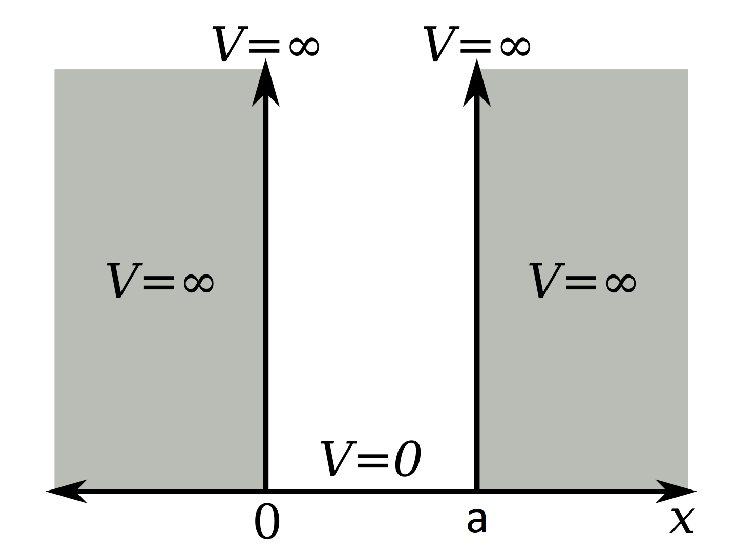
\includegraphics[width=0.4\textwidth]{./assets/Puits de Potentiel Infini.png}
  \caption{Puits de Potentiel Infini}
  \label{fig:Puits de Potentiel Infini}
\end{figure}

Montrons d'abord que $\psi (x) = 0$ dans la région où $V(x) \to \infty$. 

\begin{myproof}{}{}
Lorsque $E< V_0$, $\widetilde \psi = \gamma e ^{-qx}$, on obtient le longueur caractéristique : 
\begin{equation}
  l = \frac{1}{2q}  = \frac{\hbar}{2 \sqrt{2m (V_0 -E)}}  \underset{V_0 \to \infty}{\longrightarrow}  0
\end{equation}

\end{myproof}

\subsubsection{État stationnaire} % (fold)
\label{sec:État stationnaire}

% subsubsection État stationnaire (end)

Dans la région $x \in [0,a]$ : 
\begin{equation}
  \hat{H} \widetilde \psi = E \widetilde \psi \implies \widetilde \psi = \alpha_1 e ^{ikx} + \alpha _2 e ^{ikx} = C_1 \cos kx + C_2 \sin kx
\end{equation}

Pour conformer à des conditions limites : 

\begin{equation}
  \begin{cases}
      \widetilde \psi (0) = 0 \implies C_1 = 0 \implies \widetilde \psi = C_2 \sin kx \\ 
      \widetilde \psi(a) = 0  \implies C_2 \sin kx = 0 \implies ka = n \pi , \; n = 1, 2, \dots
  \end{cases}
\end{equation}


$k$ ne peut que prendre certain valeurs, les \textbf{énergies propres} : 
\begin{equation}
  \frac{\sqrt{2mE}}{\hbar}  = n \pi \implies \boxed{E_n = \frac{(n \pi \hbar) ^{2}}{2 m a ^{2}} , \quad n \in \mathbb{Z} ^{*}}
\end{equation}

Note : $E _{p} = E _{-p}$ pour tout $p \in \mathbb{N}$.

Les \textbf{fonctions propres (états stationnaires)} : 
\begin{equation}
  \widetilde \psi _n = C_2 \sin \frac{n \pi }{a}   x, \; n \ne 0
\end{equation}

On détermine le coefficient $C_2$ d'après la condition de normalisation : 
\begin{gather}
  \int_{0}^{a} |C_2| ^{2} \sin ^{2} \frac{n \pi x}{a}  \mathrm{d} x = 0 \\ 
  |C _ 2 | ^{2} \int_{0}^{a} \frac{1- \cos ^{2} ( n \pi x / a )}{2}  \mathrm{d}x = 1 \\ 
  |C_2| ^{2} \left( \frac{a}{2}  - \frac{1}{2}  \int_{0}^{a} \frac{\cos 2n \pi x}{a}  \mathrm{d}x \right) = 1 \\
  |C_2 | ^{2} = \frac{2}{a}  \implies C_2 = \sqrt{\frac{2}{a} }
\end{gather}

(On choisit $C_2 \in \mathbb{R}$), donc 
\begin{equation}
  \boxed{\widetilde \psi_n (x) = \sqrt{\frac{2}{a}}  \sin \left( \frac{n \pi}{a} x \right), \quad n \in \mathbb{Z} ^{*}}
\end{equation}


\subsubsection{Mesure de l'énergie} % (fold)
\label{sec:Mesure de l'énergie}

Le résultat de la mesure de l'énergie de la particule : \begin{equation}
\langle E \rangle  = \sum_{n}^{} E_n P(E_n) = \sum_{n}^{} E_n | \langle \widetilde \psi_n | \psi \rangle| ^{2} = E_n | c_n| ^{2}
\end{equation}

ou bien 
\begin{equation}
  \langle E \rangle = \langle \psi | \hat{H} | \psi \rangle
\end{equation}

\begin{myproof}{}{}
Les deux expressions sont identiques à cause de l'orthogonalité des fonctions d'ondes stationnaires.

\begin{align}
  \langle E \rangle = \int_{}^{} \psi ^{*} \hat{H} \psi &= \int_{}^{} \sum_{m}^{} c_m ^{*} \widetilde \psi_m ^{*} \hat{H} \sum_{n}^{} c_n \widetilde \psi_n \\ 
                                                        &= \int_{}^{} \sum_{m}^{} c_m ^{*} \widetilde \psi_m ^{*} \sum_{n}^{} c_n E_n \widetilde \psi_n \\
                                                        &= \sum_{m,n}^{} c_m ^{*} c_n E_n \int_{}^{} \widetilde \psi_m ^{*} \widetilde\psi_n \\ 
                                                        &= \sum_{m,n}^{} c_m ^{*} c_n E_n \delta _{m,n} \\
                                                        &= \sum_{n}^{} c_n ^{*} c_n E_n
\end{align}
\end{myproof}



% subsubsection Mesure de l'énergie (end)

\subsection{Puits de potentiel fini} % (fold)
\label{sub:Puits de potentiel fini}

\begin{figure}[H] %h:当前位置, t:顶部, b:底部, p:浮动页
  \centering
  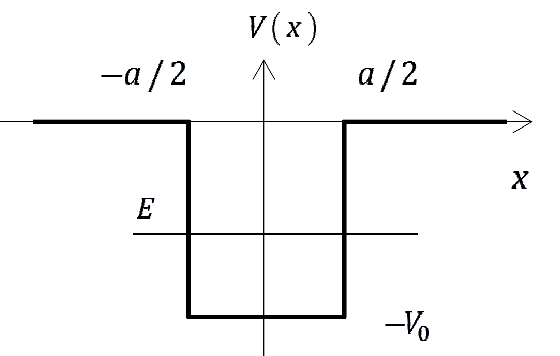
\includegraphics[width=0.4\textwidth]{./assets/Puits de Potentiel Fini.png}
  \caption{Puits de Potentiel Fini}
  \label{fig:Puits de Potentiel Fini}
\end{figure}


% subsection Puits de potentiel fini (end)



% subsection Puits de potentiel infini (end)
% section Puits de potentiel (end)
% chapter Mécanique ondulatoire (end)
